\documentclass[memoire.tex]{subfiles}

\chapter{Comment définir les critères de choix}

Afin de définir des critères pour choisir l'architecture la plus adaptée pour notre cas d'utilisation, il va falloir identifier les différentes architectures existantes pour répondre à un besoin dans le domaine du Big Data.

\section{Architecture Réactive}


\section{Architecture Répartie}


\section{Traitement des données}

Après avoir récupérer des données, nous devons passer à l'étape du traitements des données. Celui à plusieurs rôles, en effet il peut servir à formater les données, leurs apportés de la cohérence en les combinant à des données déjà présentent. Et pour finir les rediriger vers le stockage souhaité. Le traitement des données peut se faire de deux manière différentes. La première solution est le traitement par Batch, et la seconde est le traitement en temps réel~\cite{TYPE_TRAITEMENT_DONNEES}. Chacune possède ses avantages et inconvénients, nous allons voir ça plus en détails.

\subsection{Batch}

Le traitement par Batch, consiste à traiter un important volume de données à un instant T. Le traitement par batch est surtout utilisé dans les cas ou nous avons des données stockés de manière journalière, et que nous avons besoin de tout traités en fin de journée. Il n'est pas rare de voir des tâches de traitements par Batch s'exécuter dans la nuit, étant donnée que l'on traite une masse de donnée importante, on sollicite la machine pendant une longue période. Réaliser ce traitement durant des périodes creuses permet de largement diminuer l'impact sur l'utilisation de la plateforme.

\begin{figure}[!h]
	\centering 
	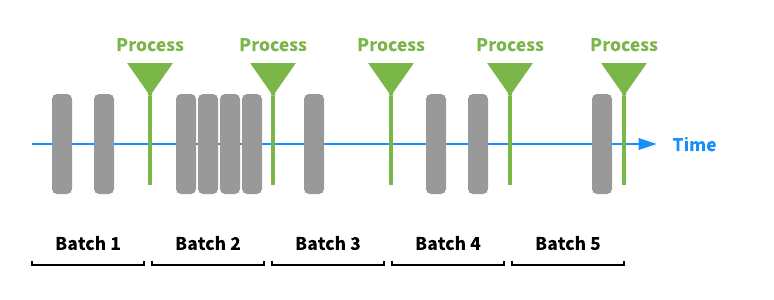
\includegraphics[scale=0.50]{img/batch-processing.png}
	\caption{Schéma du traitement par batch}
	\label{Traitement Batch}
\end{figure}


\subsection{Temps Réel}

Un traitement de données est considéré comme étant en temps réel si il s'effectue en une seconde ou moins après la réception de la donnée. Il peut être de deux types, soit des micro batchs soit en streaming.

\subsubsection{Micro-Batch}

Le traitement par micro batch est basé sur le même principe que le traitement par batch, à l'exception qu'il s'exécute beaucoup plus régulièrement (Toutes les secondes ou moins) et que le nombre de données à traiter est donc significativement plus faible. Le micro batch est surtout utilisé dans les cas où notre système ne peut pas directement réagir lorsqu'une donnée arrive, on va donc récupérer les données très régulièrement afin de garantir un traitement en temps réel ou du moins dans le délai le plus bref possible.

\subsubsection{Streaming}

Le traitement en streaming s'appuie sur l'architecture réactive. En effet, contrairement aux traitements par batch et micro batch, ici on ne vas pas récupérer des données de temps en temps. Dès qu'une donnée arrive on va la récupérer et la traiter immédiatement. De par son fonctionnement le traitement en streaming ne nécessite pas de stockage en amont contrairement aux autres type de traitement.

\begin{figure}[!h]
	\centering 
	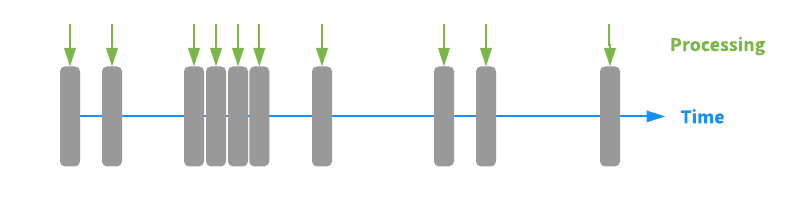
\includegraphics[scale=0.50]{img/stream-processing.png}
	\caption{Schéma du traitement en streaming}
	\label{Traitement streaming}
\end{figure}

De manière générale, on peut pas forcément se permettre de n'utiliser que l'un de ces deux type de traitement de données, nous avons régulièrement besoin de les utiliser en même temps. Des architectures ont justement été pensées pour cela~\cite{LAMBDA_KAPPA}.

\subsection{Architecture Lambda}

L'architecture Lambda a été crée dans le but de pouvoir à la fois traiter des données en batch et en streaming. Plus précisément, l'architecture lambda est composé de deux couches afin de gérer à la fois les batch et le streaming. Une couche est dédié pour traiter les données par batch, pour ensuite les rendre disponible (Ce qui est appelé une "view"). L'autre couche, s'occupe du streaming. Et à chaque donnée traitée, le résultat est mis à disposition. Grâce à ce fonctionnement lorsque l'on souhaite faire une requête, elle va pouvoir prendre en compte nos données récupérées par batch et par streaming.

\begin{figure}[!h]
	\centering 
	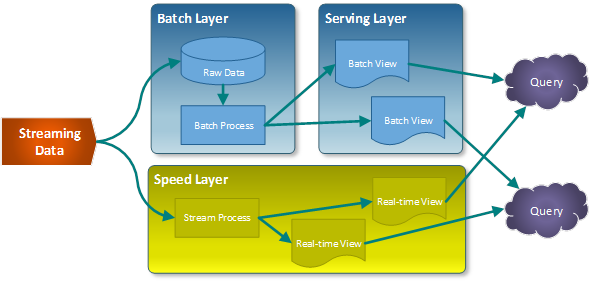
\includegraphics[scale=0.90]{img/lambda.png}
	\caption{Schéma de l'architecture Lambda}
	\label{Lambda}
\end{figure}

\subsection{Architecture Kappa}

L'architecture Kappa, se veut plus "simple". Le but étant de traiter toutes les données en streaming. Cela a pour conséquence de n'avoir qu'une seule couche contrairement aux deux nécessaire pour l'architecture Lambda. Mais cela ne permet pas de remplacer l'architecture Lambda, en effet il faut que les données que l'on récupère en Batch et la manière dont elles sont stockées, permettent de les traiter en streaming par la suite.

\begin{figure}[!h]
	\centering 
	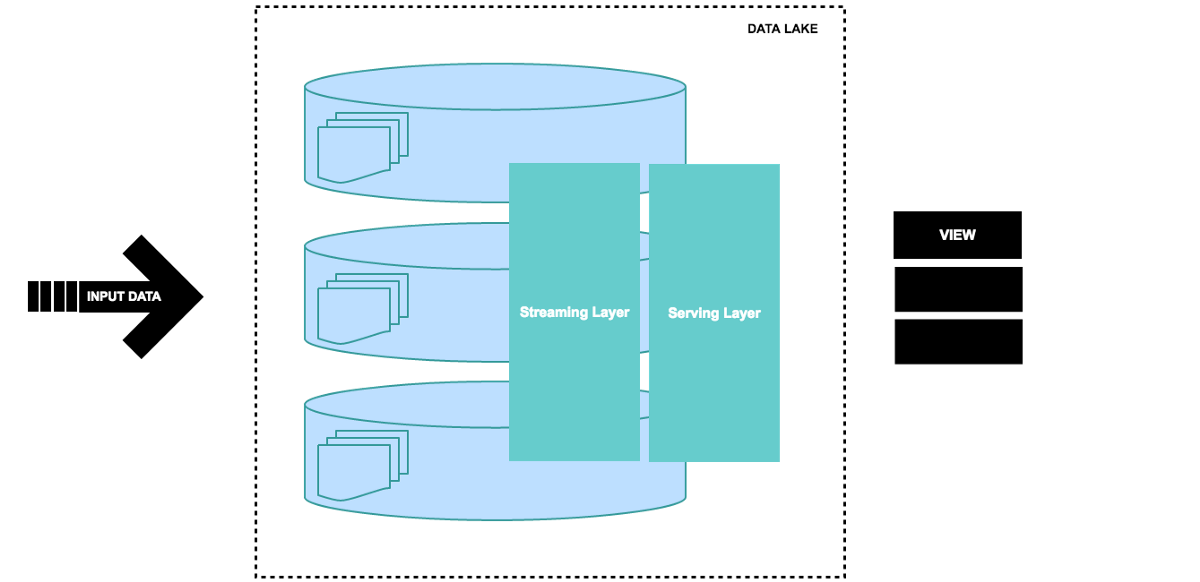
\includegraphics[scale=0.90]{img/kappa.png}
	\caption{Schéma de l'architecture Kappa}
	\label{Kappa}
\end{figure}


\section{Stockage des données}

